\chapter{Dataset and Preprocessing}
\label{ch:dataset}

\section{Dataset}

The dataset used in this project is the \textit{AI-ArtBench} dataset from Kaggle \cite{aiartbench}.
It contains over $180000$ images, of which $60000$ are human-drawn and the rest are AI-generated.
The images are pre-split into train and test data, with around $155015$ and $30000$ images used for training and testing, respectively.
Further, the dataset is divided into different subfolders, each containing images from a different epoch.
Those epochs are: Art Nouveau, Baroque, Expressionism, Impressionism, Post-Impressionism, Realism, Renaissance, Romanticism, Surrealism, Ukiyo-e. \\

\section{Preprocessing}

It should be noted that the AI generated images in this dataset were generated using two different models, Latent Diffusion (LD) and Standard Diffusion (SD).
The exact machinations of those models are not relevant here, nor is it our aim to differentiate between them.
Thus, the AI-generated images were thrown together into a single category.
Another minor change made to the dataset was to cap all folders at $5000$ images, at least before fusing the LD and SD folders.
This is the number of images for the folders containing the human drawn art.
While the inconsistency in the number of images per epoch was minute, we thought it sufficient to sacrifice a few images for the sake of stability. \\

Additionally, some images had to be resized, as, contrary to what the dataset's description claims, some images were indeed not square $256 \times 256$ images,
but rectangular instead.
Those images were cropped to $256 \times 256$ pixels and, together with the square images, randomly transformed in order to counteract overfitting later.
These transformations included horizontal flipping, rotation, zooming, shifting as well as shearing. 
Lastly, the transformed images were randomly shuffled into training and validation data and normalised by the number of pixels to avoid possible issues with numerical stability.

\begin{figure}[H]
    \centering
    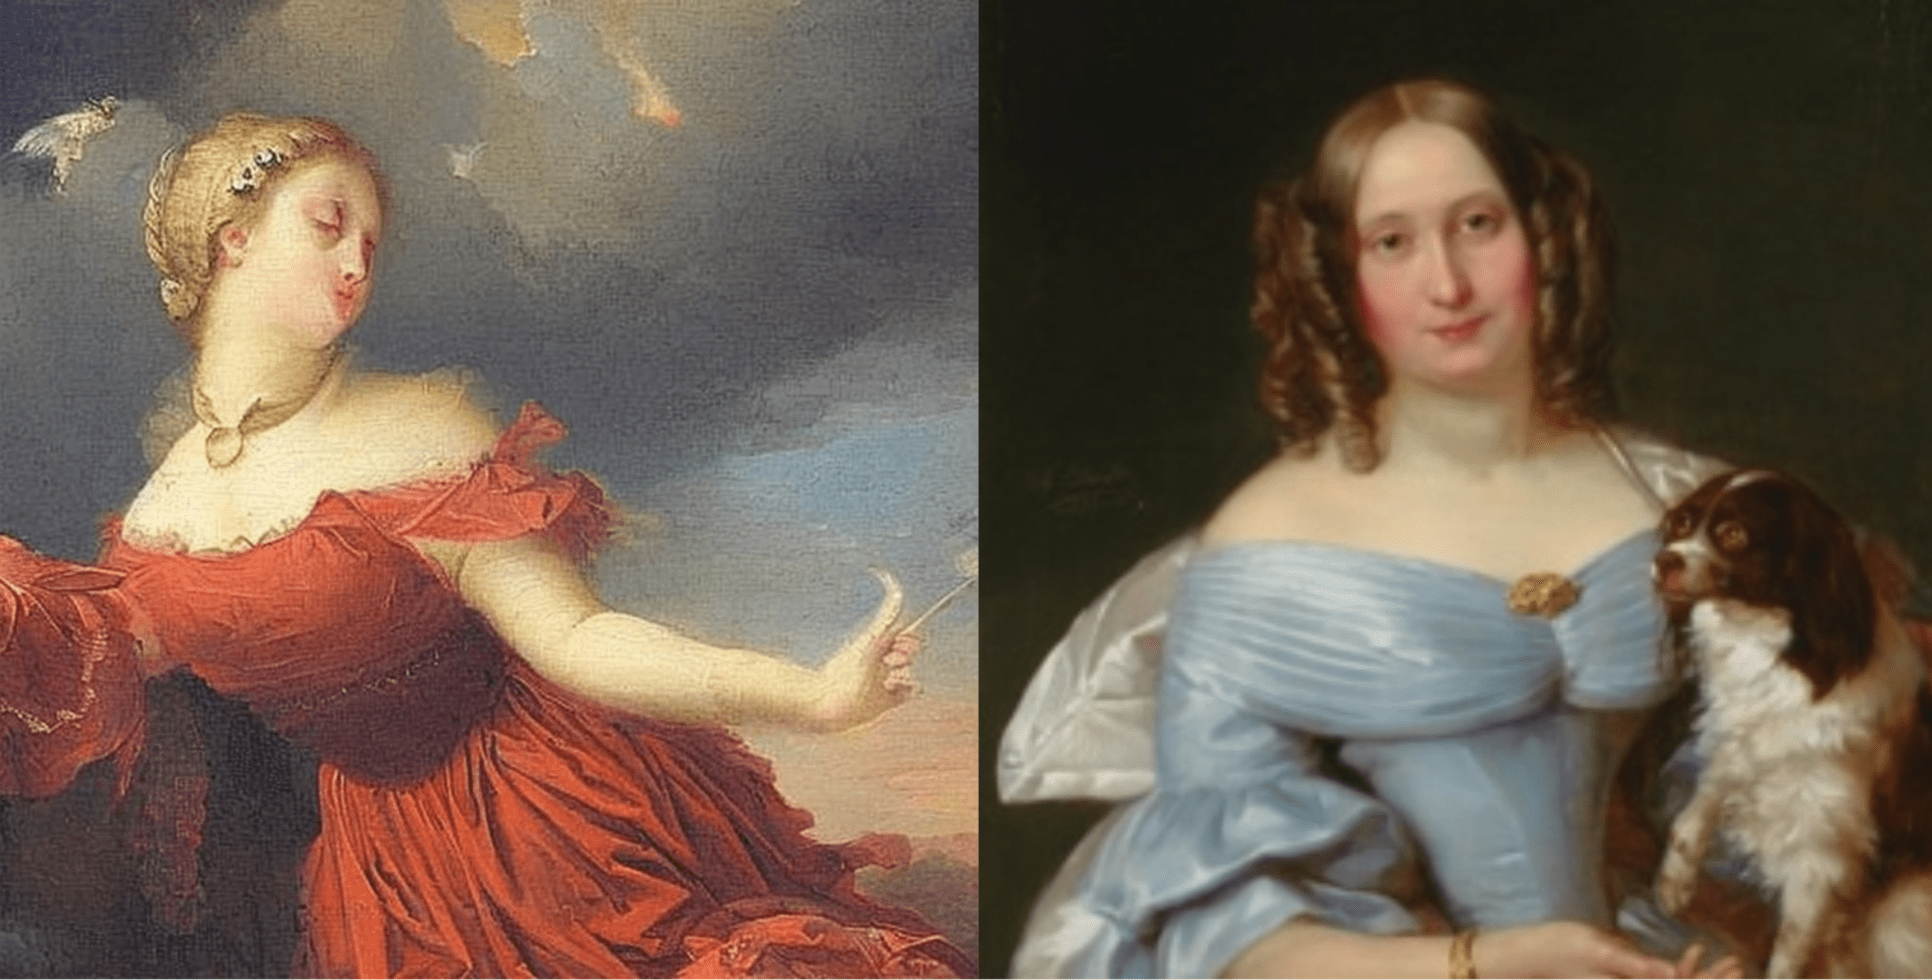
\includegraphics[width=0.5\textwidth]{images/Example_images.png}
    \caption{Example images from the dataset with the AI generated image on the left and the human-drawn on the right \cite{aiartbench}.}
    \label{fig:example_images}
\end{figure}

\section{Related Work}

The task of image classification using neural networks is perhaps the most cliché machine learning tasks.
One of the most successful and well-known models is the deep convolutional model \texttt{VGG16} \cite{VGG16source}, which will play a role again later.

When it comes to AI-image recognition, a lot of the work is done to differentiate between AI generated and real photographs (e.g see \cite{photos_example}).
We found one work on this exact dataset by Kaggle user \textit{nibrastuhh} \cite{useraiartbench}, who used
a neural network to classify the images, reaching an accuracy of over $90\%$.
They, however, focused on merely the classification of the images, while we are going to go much more in depth than they did.


